\chapter{General Analysis Strategy}
\label{chap:AnaStrategy}
\section{General R-Parity Conserving SUSY Search Strategy}

\indent In R-parity conserving SUSY searches, the sought-after super-symmetric particles are produced in pairs.  Each particle decays via a chain that ends in a stable, lightest super-symmetric particle (LSP).  If the LSP is weakly interacting, it can not be directly detectable by the ATLAS detector and must be inferred from transverse momentum conservation as \MET.  The rest of the products from the decay chain will be a series of SM particles.  ~\\

\indent All searches must distinguish between signal SUSY processes and background SM processes that mimic the signal detector signature.  Traditional search methods often place a special emphasis on identifying the LSP as this is the one decay product that is unique to SUSY events.  Practically this generally means searching for events with large amount of \MET.  \\

\indent In regions with a large mass splitting between sparticle and LSP, the decay of the original sparticle generates large amounts of momentum for the LSP.  Traditional searches therefore target the large amount of $\MET$ generated by the LSP as a method to separate signal from background. ~\\

\indent Searches isolate signal by using this and other kinematic differences.  Selections are made on sensitive variables forming a signal region (SR).  The expected background rates in SR are predicted using a combination of MC and data driven techniques.  One common technique involve making kinematically similar control regions (CR) and validation regions (VR). The CRs and VRs are designed to mimic the background kinematics in SR but are orthogonal to SR and are low expected signal rate.  We directly measure the rate of background in kinematically similar CRs and use simulation to extrapolate between CR and SR.  VRs form an independent cross check on these background predictions. \\

\indent The data in SR is originally blinded to avoid any bias for or against discovery.  We unblind the SR only after we decide the background prediction in SR is well understood based on observations in CRs and VRs. \\

\section{General Strategies in Compressed Regions}

\indent When the mass splitting between the original sparticle and its decay products becomes small, the sparticle has little energy to generate momenta in its decay products.  The result is LSPs with low momenta.  The traditional strategy of searching for events with large amount of $\MET$ therefore fails in this region of parameter space.  This problem is ubiquitous to all regions with small mass splittings.  We refer to all such regions as compressed regions.  ~\\

\indent  In our analysis, the super-partner of the top, the stop is expected to decay into a neutralino and top.  When the stop mass is close to that of the top mass plus the neutralino mass, both the top and neutralino gain very little momenta from the decay.  The invisible neutralinos in turn generate very little missing transverse energy.  This leaves only the visible tops which are mimicked by SM ttbar. \\

\indent Traditional search methods depend on variables that are highly correlated with the total magnitude of $\met$ such as $m_{T2}$ and $m_{eff}$.  Therefore traditional methods fail to separate stops from SM ttbar which has 50 to 300 times the production cross-section of stops in the region of interest.  A High-Luminosity LHC study projects a 2$\sigma$ exclusion limit up to a stop mass of 500 $\gev$ with 300 $\ifb$ of data in this region.\cite{HLLHC_stop} The projected p-value as a function of stop mass for 300 and 3000 $\ifb$ of data is given in figure \ref{fig:HL_LHC:p_value} \\

\begin{figure}[h!]
  \centering
	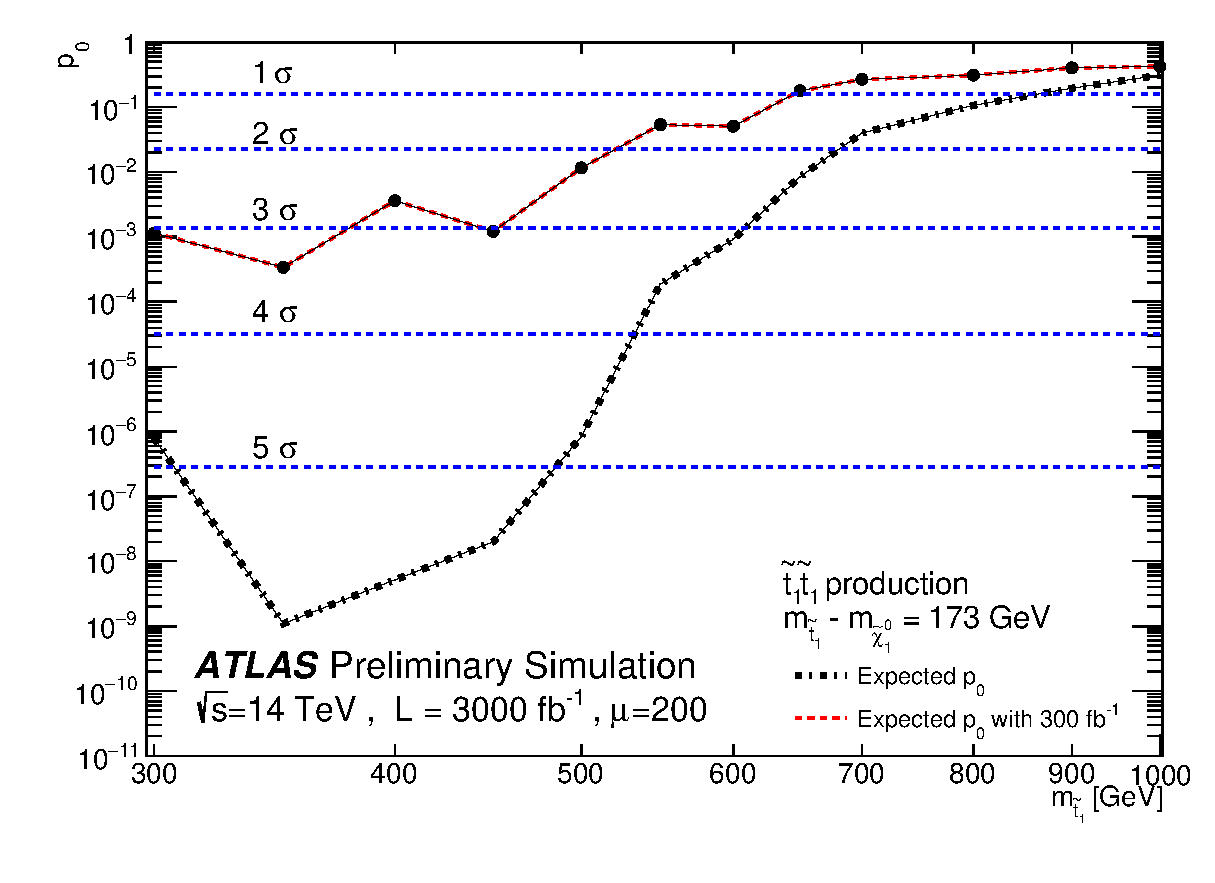
\includegraphics[width=0.65\textwidth]{./figures/strategy/HLLHC_pvalue.eps}
\caption{Projected HL-LHC sensitivity to the $\Delta m = m_t$ region with 300 and 3000 $\ifb$ of data.  Sensitivity is quantified in terms of the p-value $p_0$.  2 sigma exclusion is reached for stop masses below 500 $\gev$ with 300 $\ifb$. Figure taken from \cite{HLLHC_stop }}
\label{fig:HL_LHC:p_value}
\end{figure}

\indent However, the soft decay products can gain additional momenta if the entire system is boosted by strong initial state radiation (ISR).  The goal of the traditional searches have always been to identify the presence of the LSPs and use their presence to distinguish between signal and background.  Instead of targeting events with large amount of \MET, we use the correlations between the LSP momenta and any ISR jets to identify LSPs in compressed regions.\cite{Pheno1,Pheno2}  Because LSPs gain little momenta from stop decays, the correlation between ISR and LSPs in compressed regions tend to be extremely strong.  By targeting the correlations between ISR and $\met$ instead of the total magnitude of $\met$, we effectively turn a weakness of the compressed region into a strength. \\

\indent The relationship between the decay products and ISR also has an additional benefit of being model independent.  This correlation is dictated solely by relativistic kinematics rather than the underlying QFT of any particular model.  The direction and magnitude of the momenta of the decay products are determined mostly by two things, how heavy the decay products are and how hard they are kicked by the ISR. For the $p p \rightarrow \antibar{\stop} \rightarrow t\ninoone\tbar\ninoone$ process, the relationship is given by equation \ref{eqn:theory_MET_ISR}. This ratio between the invisible decay products and the total ISR $\pt$ is called \RISR. \\

%\begin{equation}
\begin{align}
\MET \equiv p_{\ninoone\ninoone,~T}^{~\mathrm{lab}} \sim \gamma_{\stop\stop}^{~\mathrm{lab}} \beta_{\stop\stop}^{~\mathrm{lab}} E_{\ninoone\ninoone}^{~\stop\stop} 
\sim \frac{\PTISR}{m_{\stop\stop}} 2\gamma_{\stop}^{\stop\stop} m_{\tilde{\chi}} \sim
\PTISR \frac{ 2\gamma_{\stop}^{\stop\stop} m_{\tilde{\chi}} }{ 2\gamma_{\stop}^{\stop\stop} m_{\stop} } \sim
\PTISR \frac{m_{\ninoone}}{m_{\stop}}\implies\\
\RISR \equiv \frac{\MET}{\PTISR} \sim \frac{m_{\ninoone}}{m_{\stop}}~,\quad\quad\quad\quad\quad\quad\quad\quad\quad\quad\quad\quad
\label{eqn:theory_MET_ISR}
\end{align}
%\end{equation}

\indent The ratio between \MET and ISR $\pt$ is proportional to the ratio between the mass of a single LSP and original sparticle.  Its interesting to note that the back to back boost between the two original stops does not affect the correlation between the observable \MET and ISR $\pt$.  Although the LSP's can individually gain momenta from the back to back boost of the sparticles against one another, the back to back momenta will exactly cancel resulting in zero measurable $\MET$.  \\

\indent The di-LSP system only gains $\pt$ by inheriting it from the boost by the ISR system on the two sparticles.  The fraction of the momenta that is inherited by the di-LSP system is exactly $\frac{m_{LSP}}{m_{sparticle}}$ if the sparticle decay gives no additional momentum to the LSP.  \\

\indent Figure \ref{ig:stop_400_227_ISR_MET_truth} shows the correlation between the $\RISR$ ratio in $p p \rightarrow \antibar{\stop} \rightarrow t\ninoone\tbar\ninoone$ simulation for two different stop masses (350 and 550 $\gev$) as predicted by equation \ref{eqn:theory_MET_ISR}.  The $\Delta m$ between stop and neutralino is $173 \gev$ or 550 $\mev$ from the top mass in both cases.  Both stop samples sharply peak at exactly $m_{\ninoone}/m_{\stop}$ with a gaussian width of approximately 4 percent.  No detector resolution effects were included in the simulation and only the all hadronic decay channel was considered. \\

\begin{figure}[h!]
  \centering
	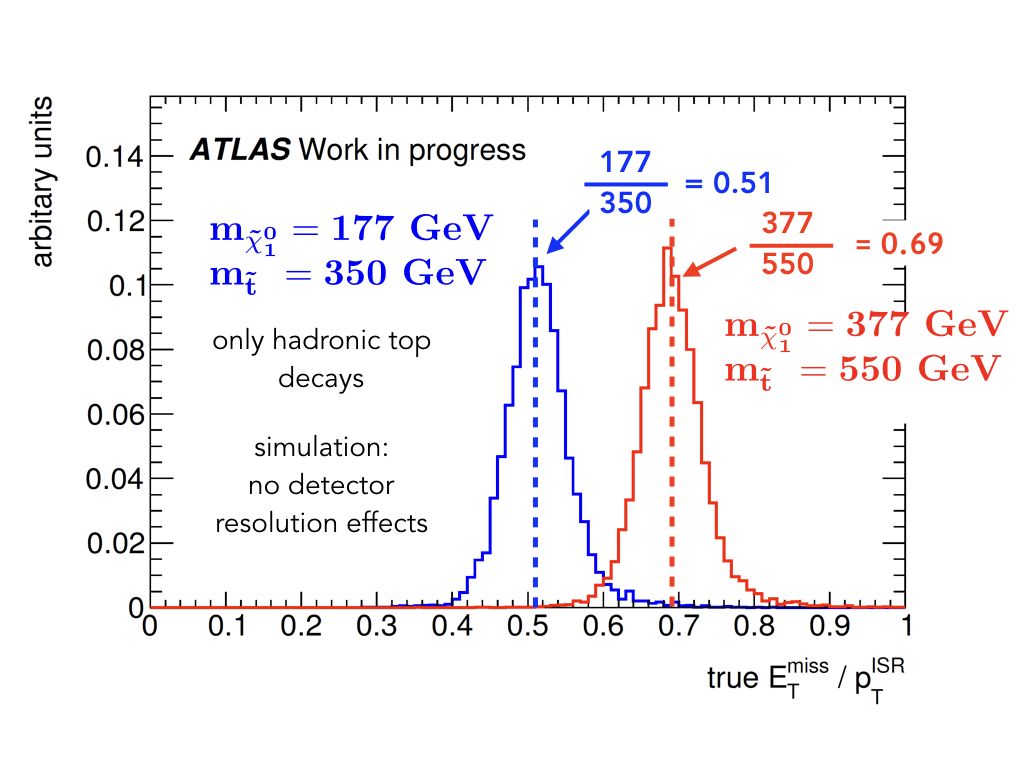
\includegraphics[width=0.65\textwidth]{./figures/strategy/RISR_truth.png}
\caption{Correlation between the $\RISR$ ratio in simulation for two different stop masses.  Both stop samples peak sharply at $m_{\ninoone}/m_{\stop}$ with only a gaussian width of 4 percent.  Deviation from the preferred ratio is limited by the top width, as the top must be pulled off-shell to generate phase space. No detector resolution effects where included and only the all hadronic decay channel was considered.}
\label{fig:stop_400_227_ISR_MET_truth}
\end{figure}

\indent The separation power of ISR and $\met$ correlations are made even stronger considering the correlation is in 2 dimensions, in magnitude and direction.  ISR and $\met$ are necessarily back to back in signal.  In comparison, the neutrino gains significant momentum directly from the top decay in ttbar background and their correlation with ISR is not as absolute.  \\

\indent By constructing variables that capitalize on this correlation we are able to separate signal from SM backgrounds.  At the same time, the increase in center-of-mass energy from 8 to 13 TeV can mean up to an order of magnitude increase in the production cross-section of signal plus strong ISR.  The 13 TeV dataset presents a golden opportunity to search for many experimentally difficult physics processes that need a boost from strong ISR in order to be detected. \\